\chapter{畳み込みアクセラレータの実装}
\section{概要}
この章ではFiC-SW1ボード上のFPGAに実装される畳み込みアクセラレータについて解説を行う。
この畳み込みアクセラレータは、図\ref{fig_cnn_on_sw1}のような並列畳み込み演算をより効率的に行う目的で実装する。
アクセラレータの大まかな設計としては、図\ref{fig_cnn_on_sw1}の処理と同様に、前の層からすべての特徴マップを入力として受け取り、分割された重みデータで並列演算し、
次の層へ特徴マップを出力するという方針を取る。

また、アクセラレータ内のすべての特徴マップ・重み・バイアスのデータは32bitの浮動小数点数で扱うものとする。

FPGA上の演算・メモリのリソースは有限なため、効率的にリソースを使用して実行サイクル数を減らさなくてはならない。
今回の設計では、アクセラレータ間でのリソース共有は行わず、各畳み込み層とアクセラレータモジュールは完全な1対1の関係になるものとした。
リソース共有を行うクロスレイヤーな設計では、並列演算性能とリソース消費をトレードオフにすることができるため、リソース消費を抑えた設計を
考える場合には有効である。

\section{アクセラレータモジュール}
図\ref{hw}に、今回実装したアクセラレータモジュールの概略図を示す。アクセラレータモジュールは大きく分けて、演算モジュール、バッファ、入出力ストリームでの3つのパートから構成される。

畳み込み演算の核となる演算モジュールは、パイプライン化された並列積和演算器(PE : Processing Elements)であり、毎サイクル、複数チャンネルの特徴マップを出力できる。
この演算モジュールは、優れた計算効率を出したUCLAのMulti-Layer CNN Accelerator\cite{fpgaopt}の設計を参考にした。

アクセラレータモジュール内のバッファは特徴マップのための入出力バッファと、重みのための重みバッファの2種類がある。
入出力バッファは、自身の演算に必要な特徴マップを格納するためのストレージで、それぞれのバッファはそれぞれの特徴マップをすべて格納できるサイズを持つ。
また、演算モジュールに毎サイクル特徴マップを入出力するために、複数個のバンクに分けることで帯域幅を確保している。
重みバッファはカーネルを格納するためのストレージで、並列化によって分割された重みのすべてを格納できるサイズと、広い帯域幅を持つ。

アクセラレータモジュールの入出力には、Xilinx社のIPであるAXI4-Streamを利用した。AXI4-Streamでは、毎サイクルNbitのデータをストリーム形式で送受信行うことができる。
今回は1サイクルで1個の32bit浮動小数点数データを送受信行える、N=32bitでのストリームとした。

\cite{fpgaopt}では高位合成を用いてスケーラブルに実装可能なアクセラレータの設計を提示している。
リソースと実行時間をトレードオフにすることができる設計を用いることで、リソース制約下で畳み込み演算の並列性を最大限活用でき、
効率的なハードウェアにすることができると考えられる。

\begin{figure}[ht]  
 \begin{center}   
   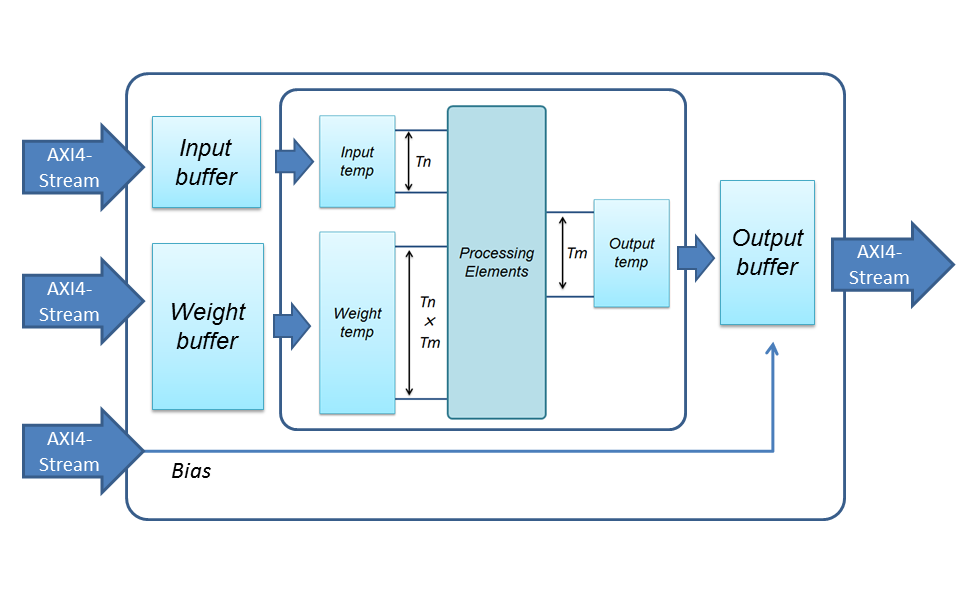
\includegraphics[bb=0 0 720 420, width=1.0\columnwidth]{img/hw.png}
  \caption{アクセラレータの概略図}
%  \ecaption{Static analysis result of an example pattern}
  \label{hw}  
 \end{center}
\end{figure}


 \subsection{演算モジュール}
この節では畳み込み演算の並列性に沿って最適化された演算モジュールを設計する。演算モジュールは、実際に計算を行う並列積和演算器PEsと、そのための一時バッファ(temp buffer)から構成される。

図\ref{pe}は並列積和演算器PEの概要である。図\ref{fig_conv}のように、畳み込み層の特徴のひとつとして、その多くの処理が入力と重みの積和演算から構成されるという点が挙げられる。
この処理の高速化には複数個の積和演算器を並列に配置するのが最も単純で効率的な方法だと考えられる。
したがって、演算モジュールはTn個の入力値からTn×Tm個の重みを用いてT個の出力値を並列に計算できる汎用的な設計となった。
さらに、スループット向上のためにPE内部はパイプライン化されており、毎サイクルTm個の値を出力バッファへと出力することができる。

パラメータTm、Tnはそれぞれ、PEsが同時に扱う入力データ、出力データの数であり、リソース消費量とトレードオフ関係にあるため実装最適化の対象となる。
今回の設計では暫定的に演算モジュールのサイズは(Tm, Tn)=(24, 8)に固定したが、リソース上限によってはこのパラメータを変更することでリソース上限内に消費量を
抑えることが必要となる。

PEsの入出力は演算モジュール内の一時バッファ(temp buffer)に保存される。一時バッファは、入出力バッファ・重みバッファとPEsの間に入り、PEsが入力データTn個、重みTn×Tm個、出力データTm個を高速に
読み書きを行うためのレジスタの役割を持つ。演算モジュール外部から見れば、それぞれ対応する一時バッファのデータを読み書きすることで、計算が行われるという流れになる。

\begin{figure}[ht]  
 \begin{center}   
   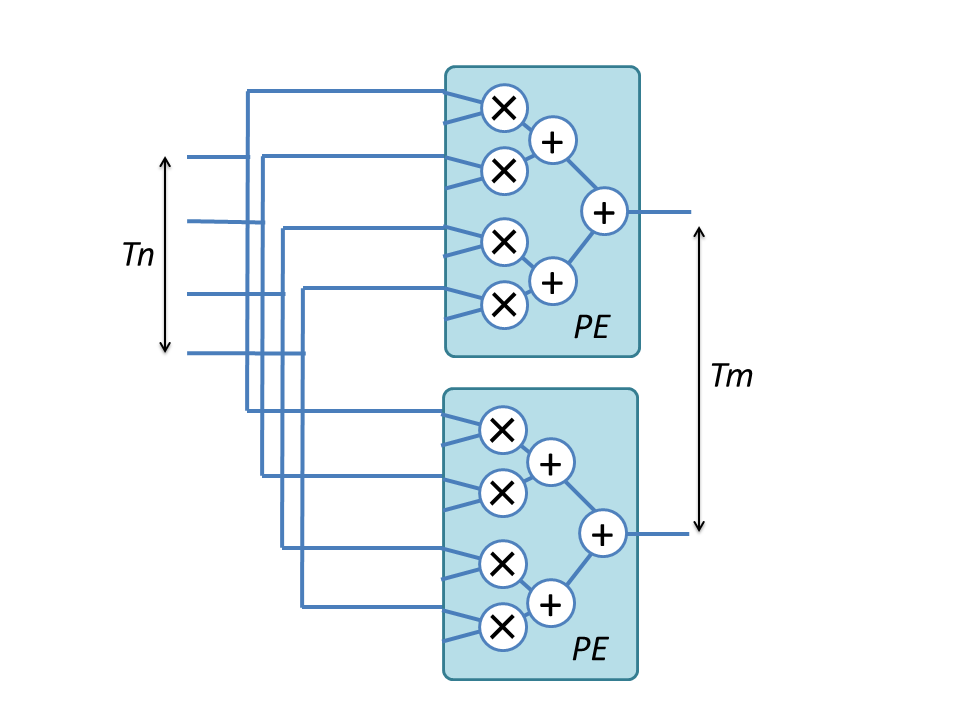
\includegraphics[width=1.0\columnwidth, bb=0 0 720 540]{img/pe.png}
  \caption{並列積和演算器PEs}
%  \ecaption{Static analysis result of an example pattern}
  \label{pe}  
 \end{center}  
\end{figure}
 
\subsection{入出力バッファと重みバッファ}
スイッチモジュールから送られてきた入力特徴マップのデータは、まずFPGA上に確保された入力バッファに蓄えられる。

高速に畳み込み演算を行うためには、演算モジュールは可能な限り広い帯域幅で入力特徴マップにアクセスできなけらばならない。
そこで、入力バッファを特徴マップごとにバンクを分割し並列に読み込むことができるようにした。
これにより、入力バッファと演算モジュールの帯域幅はTn/バンク数となり、帯域幅を改善することができる。
同様の手法で、出力バッファや重みバッファも帯域幅を増減させることができる。。

今回の実装では、入力バッファはTn個、出力バッファはTm個、重みバッファはTm×Tn個に分割することで、最大となるような帯域幅を確保した。
これにより、演算モジュールが毎サイクル、畳み込み演算を行う効率的な機構を実現した。
ただし、この実装を行う場合、バンク数に応じてFPGAリソース消費量が増大するため、過剰なバンク分割によってリソースを浪費することに注意しなければならない。

図\ref{fig_buffer}に、入出力バッファ・重みバッファを演算モジュールと接続した概略図を示す。バッファが特徴マップの次元数によって、
入力バッファはTn個、出力バッファはTm個、重みバッファはTm×Tn個のバンクに分割されている様子がわかる。

\begin{figure}[ht]  
 \begin{center}   
   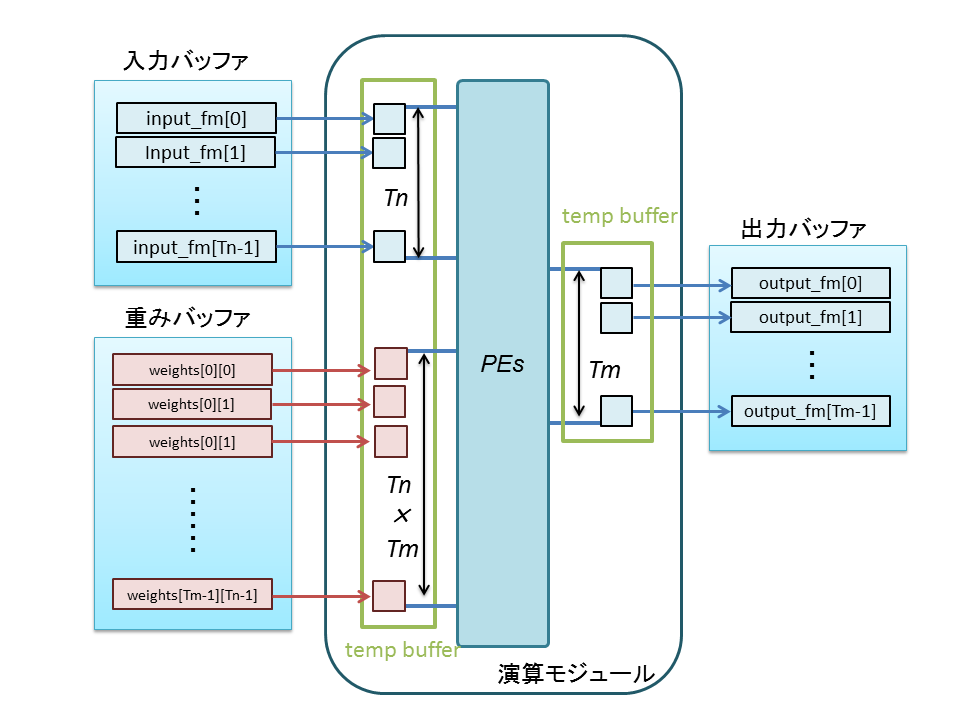
\includegraphics[width=1.0\columnwidth, bb=0 0 720 540]{img/buffer.png}
  \caption{入出力バッファ・重みバッファと演算モジュールの接続}
%  \ecaption{Static analysis result of an example pattern}
  \label{fig_buffer}  
 \end{center}  
\end{figure}